
\section{Research Process}
Part of any research process is rigorous record keeping to ensure experiments can be independently and reliably reproduced.
While researchers keep meticulous journals, when dealing with software this bookkeeping can be largely automated.


\subsection{Version Control}
Software engineering primarily relies on version control systems, such as GitHub or BitBucket, to keep track of code changes.

....

\subsection{Experiment Tracking}
\begin{figure}[h]
    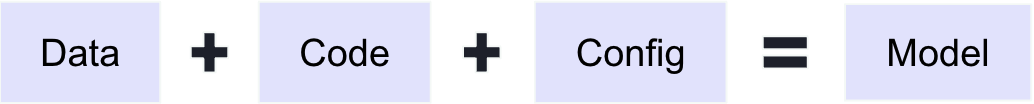
\includegraphics[width=\linewidth]{chapters/NLP/figures/model.png}
    \label{fig:model}
\end{figure}
An experiment is defined by the training code, data, and configuration.
When ML and Data Science are involved, the data generating process has to be documented.
In software engineering we say that code doesn't exist until it is "checked into" version control.
Similarly, data doesn't exist until it is stored in the cloud.
In addition to the raw data, we should also store documentation about how it was created, by whom, when, and any additional processing steps.
This should be done in a way that is easy to replicate and understand -- ideally directly in code.

Version control system are specialized to keep track changes in plain text files, but they are not well suited for tracking the other aspects of an experiment.
The ML community has developed specialized tools\footnote{Weights\&Biases, Neptune}, which we have integrated into Sheepy.
These tools are excellent at visualizing and comparing of
\begin{itemize}
    \item Hyperparameters
    \item Model metrics
    \item (Interactive) plots
    \item Logs
    \item Hardware configuration
    \item Hardware metrics
    \item Code and dependency versions
    \item Artifacts (raw data, processed data, models)
\end{itemize}
and facilitate collaboration and sharing of results by directly linking to the experiments.

At the beginning of a new training run an experiment is initialized and data related to the run streamed to a web based platform.
The next step is obtaining data artifacts from a cloud storage provider\footnote{Amazon S3, Google Cloud Storage}, preprocessing, training and finally storing and tracking of output artifacts and metadata.
Metadata can include information about how many samples the data contains, the size and type of fields, input features and outputs of a model, when it was created etc..
This facilitates discovery, analysis, iteration, and collaboration.

\subsection{Data Preparation}
We will go over each step of data preparation in the next sections:
\begin{itemize}
    \item Data download
    \item Pre-processing
    \item Splitting into training, validation, and test sets
    \item Feeding data to the model during training
\end{itemize}

The goal is to rerun an experiment from scratch with a single command and we build on top of PyTorch Lightning's \pythoninline{DataModule} class to handle these steps.
\subsubsection{Data Download}
Downloading the dataset from cloud storage and caching are handled in the \pythoninline{prepare_data} method and only executed once per run.
We will first check if the data is already cached, and if not, download it.

\subsubsection{Data Preprocessing}
Pre-processing refers to transformation steps we want to apply to the raw data to make it suitable to input into the model.
For example in NLP, raw text needs to be cleaned, tokenized, trimmed and padded (see Section \ref{vocabularies_and_words}) (Fig. \ref{fig:tokenization}).
\begin{figure}
    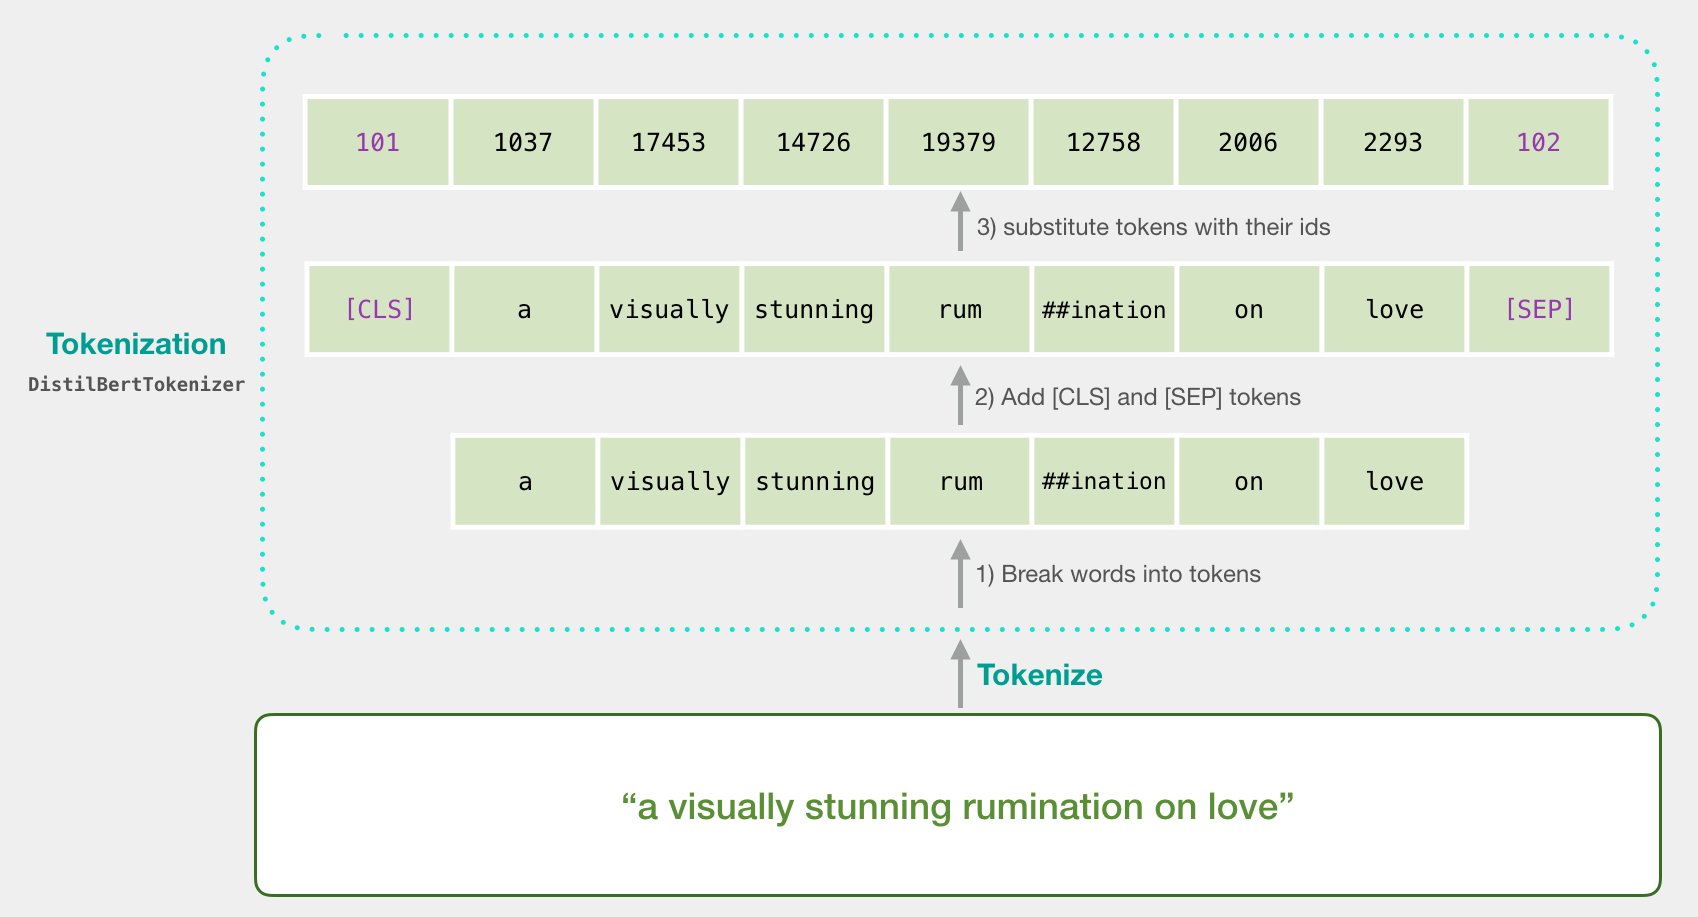
\includegraphics[width=\linewidth]{chapters/NLP/figures/tokenization.png}
    \caption{Tokenization}
    \label{fig:tokenization}
\end{figure}
These steps can be slow and in principle we need to do them only once per sample and cache the results.

\subsubsection{Data Splitting}
\begin{figure}[h]
    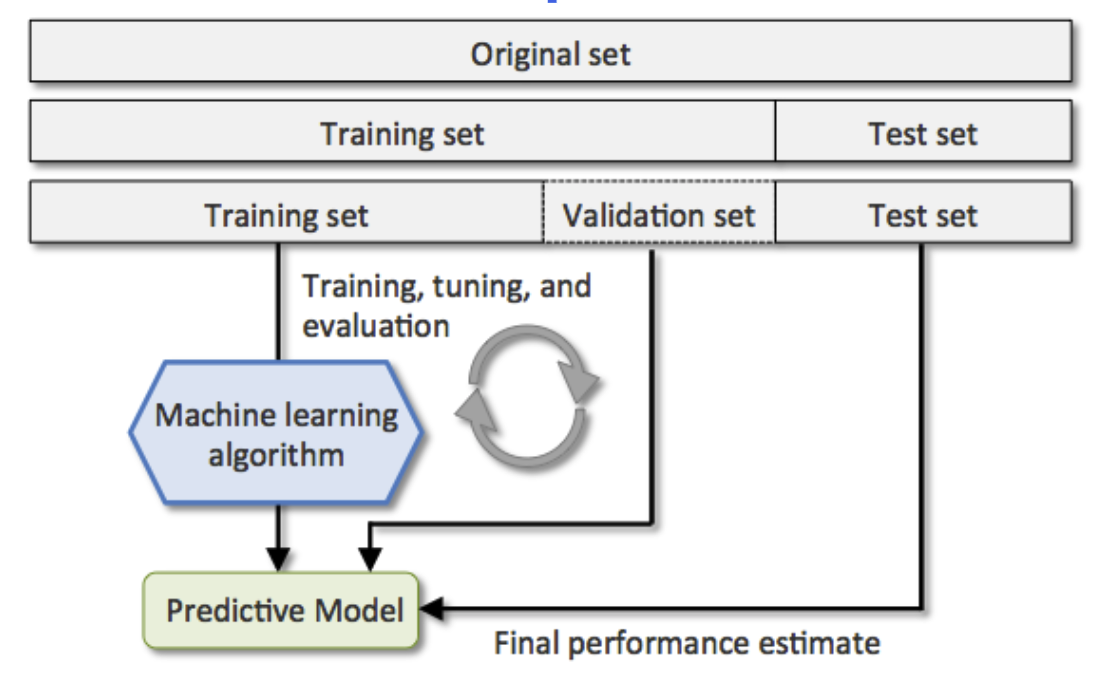
\includegraphics[width=\linewidth]{chapters/NLP/figures/data_splitting.png}
    \caption{Data Splitting}
    \label{fig:data_splitting}
\end{figure}
To evaluate the generalization performance of a model we need to test it on data it hasn't seen during training.
The dataset is therefore split into training and validation sets, usually at random (Fig. \ref{fig:data_splitting}).
It should be ensured the randomness is deterministic to reproduce results exactly, which can be achieved by setting a "seed" for the random number generator.
The validation set is used during training to monitor progress and tune hyperparameters.
In addition, it is good practice to hold out another portion of the data, the test set, which is never used during training, but only to report final results.
We otherwise run the risk of tuning hyperparameters to the validation data, thereby overestimating real performance.
While datasets are continuously evolving, we should keep a frozen version of the data to get fair comparisons.

\begin{itemize}
    \item Training dataset: Tune model parameters $\theta$ (80\% of the data)
    \item Validation dataset: Tune hyperparameters (10\% of the data)
    \item Testing dataset: Evaluate and report the performance of the model (10\% of the data)
\end{itemize}


\subsubsection{Feeding Data to the Model}
\begin{figure}[h]
    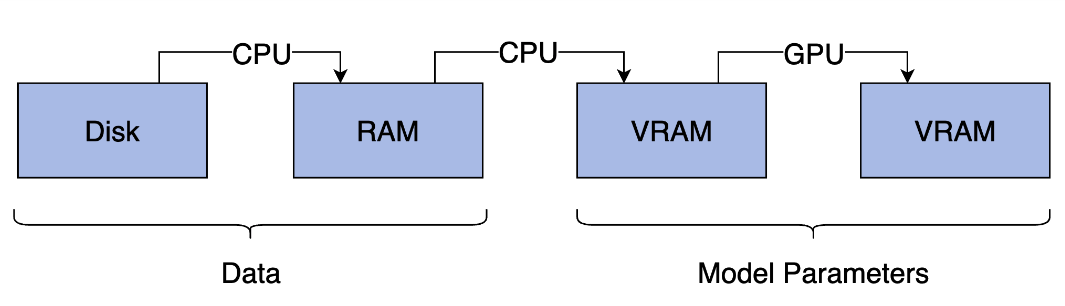
\includegraphics[width=\linewidth]{chapters/NLP/figures/ram_cpu_vram.png}
    \caption{Data needs to be moved from disk to RAM to VRAM so that it can be used to update the model parameters.}
    \label{fig:ram_cpu_vram}
\end{figure}
Model parameters are stored in GPU memory (known as VRAM); in order to update them, the GPU needs to process data from the training set.
After downloading the data from cloud storage it resides on local disk, from where it needs to be moved to RAM and finally VRAM.
Loading data into the model needs to be fast, or we run the risk of starving the GPU, meaning the GPU processes each batch of data faster than the CPU can deliver the next one, leading to low resource utilization and slow training.
We use PyTorch's \pythoninline{DataLoader} class to parallelize this process across multiple CPU workers.
A \pythoninline{DataLoader} takes as argument a \pythoninline{Dataset} and provides a stream of batches of data.
The \textit{batch size} is an important parameter that needs to be tuned on a case by case basis, as we will explain in the next section.

\subsection{Training}
\begin{figure}[h]
    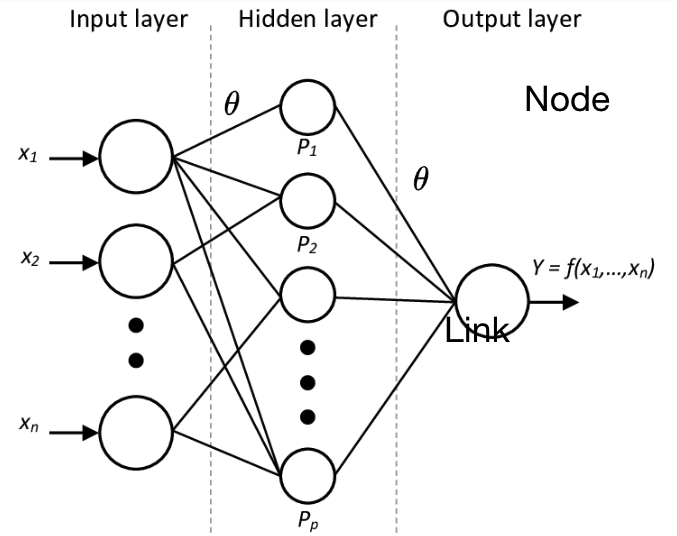
\includegraphics[width=\linewidth]{chapters/NLP/figures/model_architecture.png}
    \caption{Deep neural network architecture}
    \label{fig:model_architecture}
\end{figure}

While glossing over some details, model training can summarized in the following steps:
\begin{itemize}
    \item Given data pairs $(x_i, y_i)$, where $x_i$ is an input sample, and $y_i$ is the desired output
    \item Determine a function $f$, such that $f(\theta, x_i) = \hat{y}_i \approx y_i$, where $\theta$ are model parameters and $f$ is the model architecture
    \item Define a loss function $L(\theta) = \sum_i L(\hat{y}_i, y_i)$ that measures how close the model's output is to the desired output
    \item Optimize $\theta$ to minimize $L(\theta)$
\end{itemize}
\begin{figure}[h]
    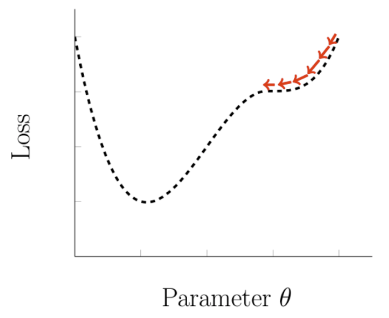
\includegraphics[width=\linewidth]{chapters/NLP/figures/loss.png}
    \caption{Minimizing the loss function}
    \label{fig:loss}
\end{figure}
Here the loss function can take on many forms, depending on the training task, we summarize some of the most common ones in Table \ref{table:losses}.
\begin{table}
    \centering
    \renewcommand{\arraystretch}{1.3}
    \begin{tabular}{|c| c| c|}
    Loss Name & Function & Use \\[0.5ex] \hline
    Mean Squared Error & $\begin{array} {lcl} \frac{1}{N} \sum_{i=1}^N|\hat{y}_i - y_i|^2\end{array}$  & regression \\ [0.5ex]
    Binary Cross Entropy & $\begin{array} {r@{}l@{}} -\frac{1}{N} \sum_{i=1}^N (y_i \cdot log(\hat{y}_i) + (1 - y_i) \cdot log(1-\hat{y}_i)) \end{array}$ & binary classification \\ [0.5ex]
    Cross Entropy & $\begin{array} {r@{}l@{}} -\frac{1}{N} \sum_{i=1}^N y_i \cdot log(\hat{y}_i) \end{array}$ & multiclass classification \\ [0.5ex]
    \end{tabular}
    \caption{Loss functions}
    \label{table:losses}
\end{table}
Parameters in the last layer are then optimized according to the rule
\begin{equation}
    \label{eq:optimization}
    \theta \rightarrow \theta - \alpha \frac{\partial L}{\partial \theta}
\end{equation}
where $\alpha$ is called the \textit{learning rate} and determines the step size, the partial derivative of the loss function with respect to the parameters is called the \textit{gradient}.
For other parameters the rule is similar, but involves the application of the chain rule from calculus.
The algorithm is called \textit{gradient descent} and is the workhorse of all modern deep learning.
In contemporary architectures there are millions to hundreds of billions of parameters, and updating them efficiently is crucial.

To optimize the parameters as outlined in Eq. \ref{eq:optimization} we need to evaluate the gradient of the loss function given the data $(x_i, y_i)$.
To compute the optimial update step we need to sum over all samples in the dataset, compute and store all the gradients, update the parameters once, and repeat the process until convergence.
This, however is not practical, given the size of typical datasets and the number of model parameters -- each step would be very computationally expensive and the training slow.

On the other end of the spectrum we could use only a single sample to compute approximations of the optimal gradients, and they will take us close to the global minimum.
This method is called \textit{stochastic gradient descent} and generally works well, but it comes with some tradeoffs:
\begin{itemize}
    \item Loading single samples from the dataset is slow, due to CPU, RAM and bus overhead when copying data to VRAM
    \item There is overhead in the GPU related to scheduling of compute operations
    \item The gradients are much more noisy than the optimal ones, and the model will learn more slowly (see Fig. \ref{fig:mini-batch})
\end{itemize}
There is a happy middle ground called \textit{mini-batch gradient descent} which is a combination of stochastic gradient descent with mini-batches.
Using mini-batches allows for a more accurate estimate of the gradient, and reduces the overhead per sample, as we can take advantage of hardware accelerated vectorized compute operations in CPUs and GPUs.
In practice, we will choose a batch size that is much smaller than the number of samples in the dataset, and as big as possible without running out of VRAM, where the latter condition is typically the more relevant constraint.

\begin{figure}[h]
    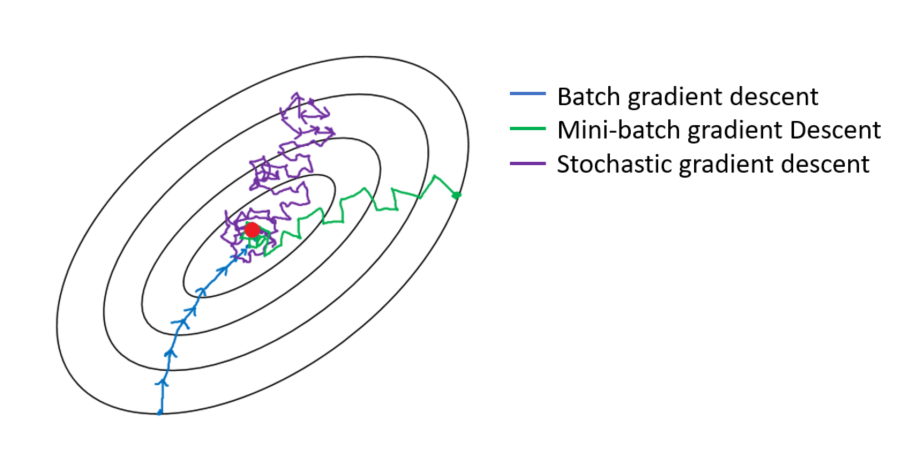
\includegraphics[width=\linewidth]{chapters/NLP/figures/mini-batch.png}
    \caption{Batch vs mini-batch vs stochastic gradient descent}
    \label{fig:mini-batch}
\end{figure}

\subsection{Evaluation and Metrics}
\label{evaluation}
To know how well our model is doing we need to define how to measure its performance.
When the target is a real number (regression) we can simply compare the model output using one of the metrics in Table \ref{table:regression_metrics}.
\begin{table}
    \centering
    \renewcommand{\arraystretch}{1.3}
    \begin{tabular}{|c| c| c|}
    Metric Name & Function & Abbreviation \\[0.5ex] \hline
    Mean Squared Error & $\begin{array} {lcl} \frac{1}{N} \sum_{i=1}^N|\hat{y}_i - y_i|^2\end{array}$ & MSE \\ [0.5ex]
    Mean Absolute Error & $\begin{array} {lcl} \frac{1}{N} \sum_{i=1}^N|\hat{y}_i - y_i|\end{array}$ & MAE \\ [0.5ex]
    Root Mean Squared Error & $\begin{array} {lcl} \sqrt{\frac{1}{N} \sum_{i=1}^N|\hat{y}_i - y_i|^2}\end{array}$ & RMSE\\ [0.5ex]
    Mean Absolute Percentage Error & $\begin{array} {lcl} \frac{1}{N} \sum_{i=1}^N \left| \frac{\hat{y}_i - y_i}{y_i}\right|\end{array}$ & MAPE\\ [0.5ex]
    Symmetric Mean Absolute Percentage Error & $\begin{array} {lcl} \frac{1}{N} \sum_{i=1}^N\frac{|\hat{y}_i - y_i|}{|\hat{y}_i| + |y_i|}\end{array}$  & SMAPE \\ [0.5ex]
    \end{tabular}
    \caption{Regression metrics}
    \label{table:regression_metrics}
\end{table}

When the target is a categorical variable (classification) we will still get a distribution of real numbers as output, i.e. the confidence of the model that a sample belongs to a certain class or set of classes.
The model output will be close to one if the sample belongs to the class, and close to zero if it does not.
To compute classification metrics, we critically need to define a \textit{threshold}.
By default we would choose $0.5$, as that corresponds to how the loss function determines whether to push a sample in on direction or the other.
Later we will discuss reasons and tips for how and why you might want to change this value.

Assuming we have only have two classes, i.e. $True$ or $False$, once a threshold has been chosen, every sample will be in one of four categories:
\begin{itemize}
    \item The model output is greater than the threshold and the sample belongs to the $True$ class, we call this a True Positive ($TP$)
    \item The model output is greater than the threshold and the sample belongs to the $False$ class, we call this a False Positive ($FP$)
    \item The model output is less than the threshold and the sample belongs to the $True$ class, we call this a False Negative ($FN$)
    \item The model output is less than the threshold and the sample belongs to the $False$ class, we call this a True Negative ($TN$)
\end{itemize}
With this we can define the metrics in Table \ref{table:classification_metrics}.
\begin{table}
    \centering
    \renewcommand{\arraystretch}{1.3}
    \begin{tabular}{|c| c| c|}
    Metric Name & Function & Interpretation \\[0.5ex] \hline
    $Accuracy$ & $\begin{array} {lcl} \frac{TP + TN}{TP + FP + FN + TN}\end{array}$ & Fraction of samples classified correctly  \\ [0.5ex]
    $Precision$ & $\begin{array} {lcl} \frac{TP}{TP + FP}\end{array}$ & Of all samples predicted as $True$, fraction of $True$ samples \\ [0.5ex]
    $Recall$ & $\begin{array} {lcl} \frac{TP}{TP + FN}\end{array}$ & Of all $True$ samples, fraction of samples predicted as $True$ \\ [0.5ex]
    $F_1$ & $\begin{array} {lcl}2\frac{Precision \times Recall}{Precision + Recall} \end{array}$ & Harmonic mean between Precision and Recall \\ [0.5ex]
    \end{tabular}
    \caption{Classification metrics}
    \label{table:classification_metrics}
\end{table}
Most classification problems are strongly imbalanced and we typically assign the $True$ label to the less common class.
This also means that $Accuracy$ is rarely the best metric to consider.
For example, assume we have an imbalance of $1 : 100$ of $True : False$, if we have an algorithm that always predicts $False$ we will get $Accuracy = 0.99$, $Precision = undefined$, $Recall = 0.00$, $F_1 = undefined$.
By adjusting the threshold we can change the tradeoff between $Precision$ and $Recall$ according to our downstream needs, reflecting whether it is more acceptable to have have a higher rate of $FP$ or $FN$ predictions.
For example, it may be acceptable to lower the threshold if the goal is finding very rare events from a large dataset for manual inspection, resulting in lower $Precision$ but higher $Recall$.
The $F_1$ score is balanced measure of $Precision$ and $Recall$ and will be low if any of them is low, and there is a threshold for which it will be maximal.
As a rule of thumb, you should aim to achieve $F_1 \gtrsim 0.7$.

There is another metric that is often used in classifcation tasks that is independent of class imbalance and threshold called the area under the $Receiver\; Operating\; Charateristic$ curve, or $ROC\; AUC$.
For this we determine the $False\; Positive\; Rate$ ($FPR$) and $True\; Positive\; Rate$ ($TPR$) for each threshold.
\begin{equation}
    FPR = \frac{FP}{FP + TN}; \;\;
    TPR = \frac{TP}{TP + FN}.
\end{equation}
You can think of the integral of the resulting curve as taking a weighted mean over all possible thresholds, see also Figure \ref{fig:roc_curve}.
\begin{figure}[h]
    \centering
    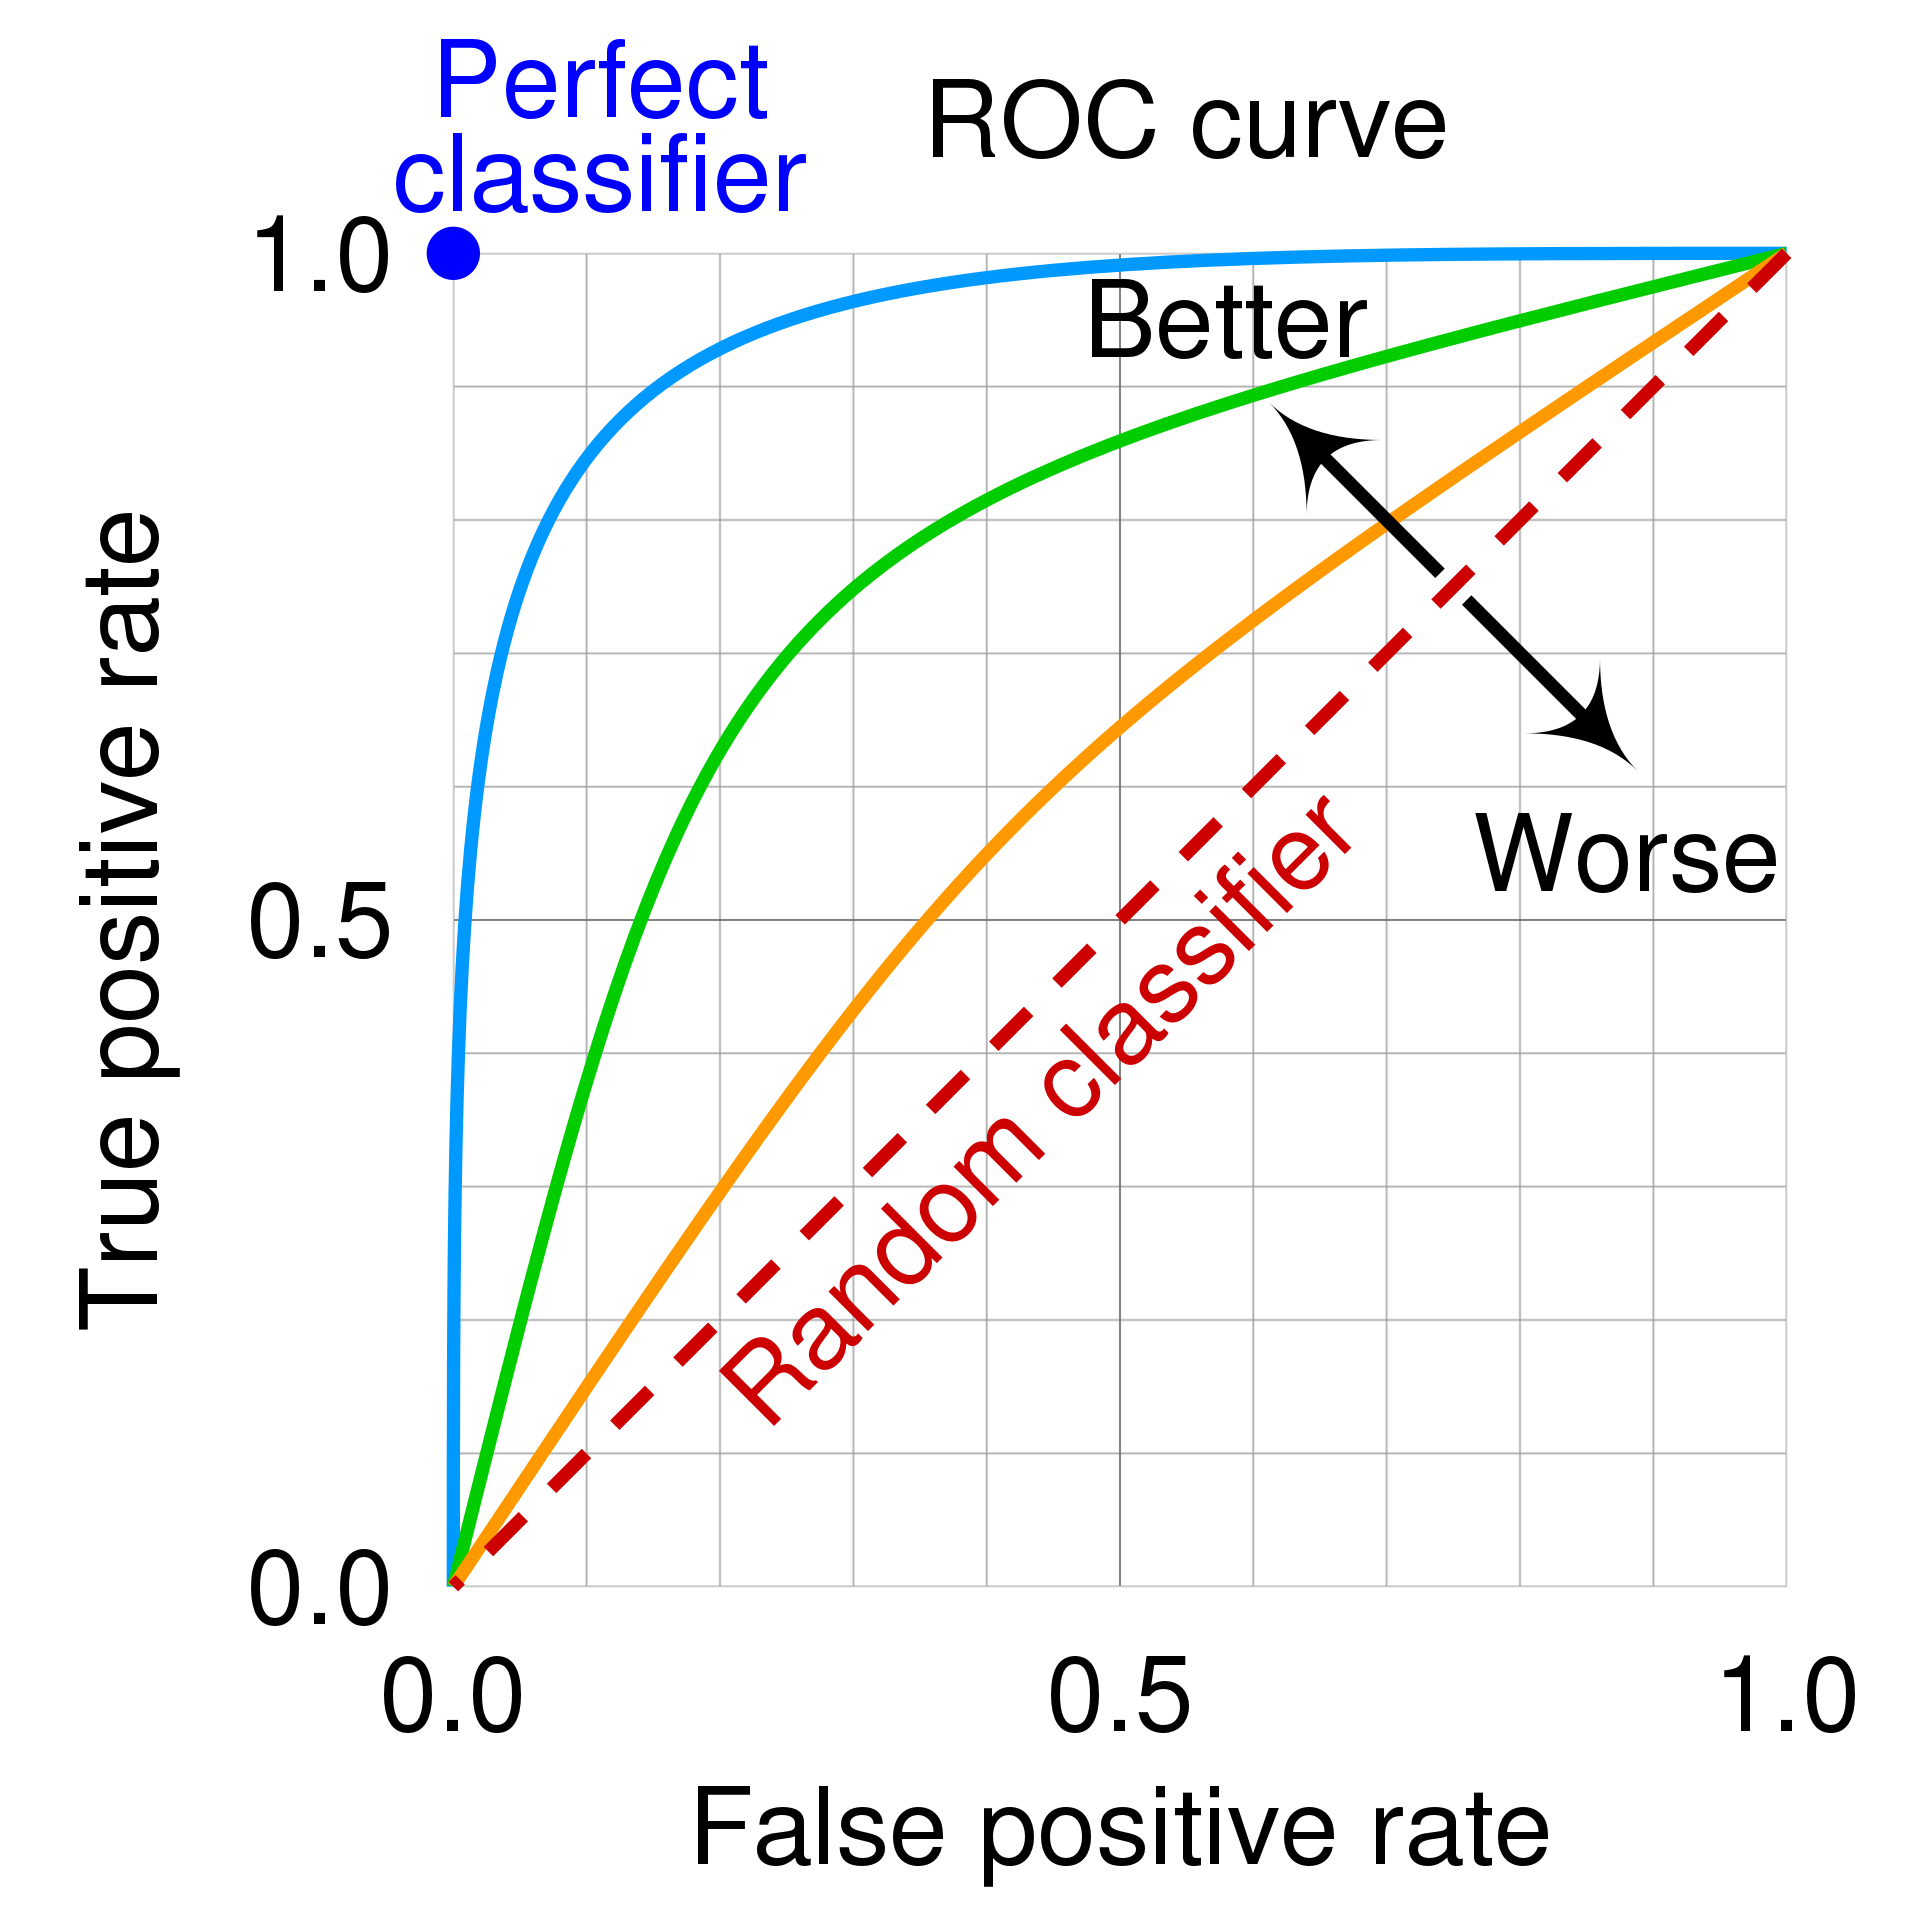
\includegraphics[width=0.8\textwidth]{chapters/NLP/figures/Roc_curve.svg.png}
    \caption{ROC curve, a random classifier would achieve $AUC = 0.5$, a perfect one $1.0$.}
    \label{fig:roc_curve}
\end{figure}

We automatically generate metrics and plots relevant for text classification tasks in the code accompanying this chapter.
